\begin{enumerate}[label=\thesubsection.\arabic*.,ref=\thesubsection.\theenumi]
\numberwithin{equation}{enumi}

\item
For a unity feedback system shown in  Fig.  \ref{fig:ee18btech11033_block}, having transfer function given below in eq \ref{eq:ee18btech11033_tf}.  Design the value of gain K for $\brak{i}$ a gain margin of 33 dB. $\brak{ii}$ Phase margin of 40\degree. $\brak{iii}$ to yield maximum peak overshoot of 20 percent for a step input.

\begin{figure}[!ht]
	\begin{center}
		
		\resizebox{\columnwidth}{!}{\input{block.tex}}
	\end{center}
\caption{}
\label{fig:ee18btech11033_block}
\end{figure}

\begin{align}
\label{eq:ee18btech11033_tf}
G\brak{s} &= \frac{K}{\brak{s+3}\brak{s+9}\brak{s+15}}
\end{align}
\solution 

\begin{align}
\label{eq:ee18btech11033_Tf(s)}
G\brak{s}H\brak{s} &=\frac{K}{\brak{s+3}\brak{s+9}\brak{s+15}}
\end{align}
For K=1 let:
\begin{align}
\label{eq:ee18btech11033_B(s)}
B\brak{s} &= \frac{1}{\brak{s+3}\brak{s+9}\brak{s+15}}
\end{align}
Gain of the given transfer function is:
\begin{align}
\label{eq:ee18btech11033_gain}
      = 20log\brak{\abs{G\brak{s}H\brak{s}}}
    \\= 20log\brak{K} +20log\abs{B\brak{s}}
\end{align}
Phase of the given transfer function is:
\begin{align}
\label{eq:ee18btech11033_phase}
      = \angle{G\brak{s}H\brak{s}}
    \\= \angle{B\brak{s}}
\end{align}
 Thus value of K has : a) no effect on phase. b) linear effect on gain.




\item $\brak{i}$ Given gain = 33dB
\\
\solution The following code generates Bode plot of $B\brak{s}$ as shown in Fig \ref{fig:ee18btech11033_1}

\begin{lstlisting}
codes/ee18btech11033_1.py
\end{lstlisting}

\begin{figure}[!ht]
\centering
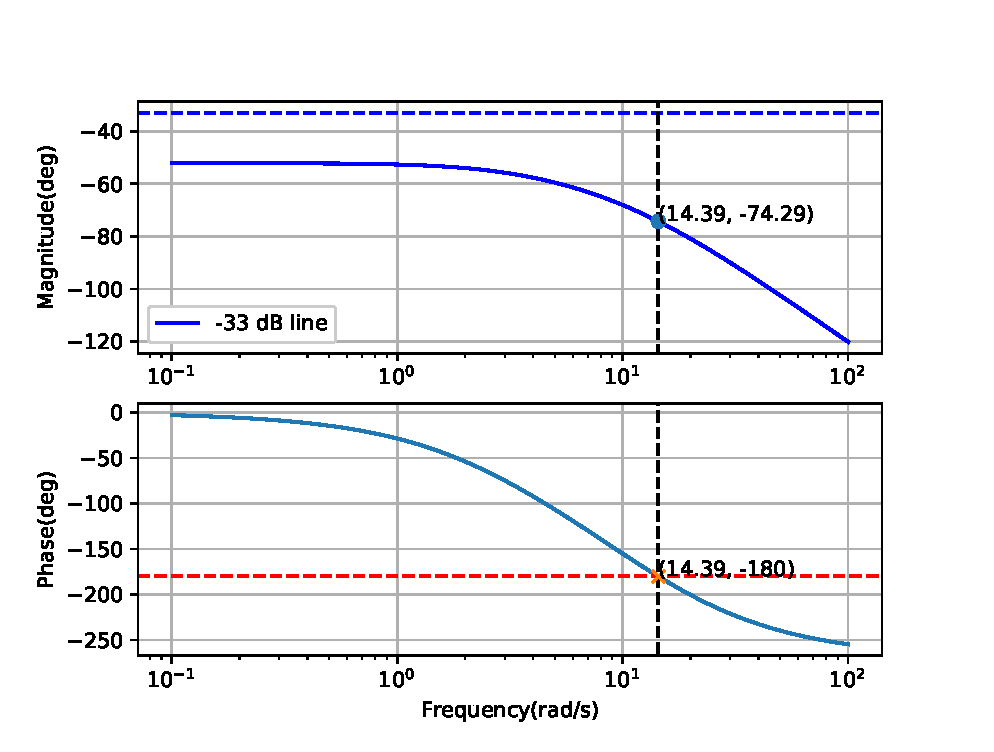
\includegraphics[width=\columnwidth]{ee18btech11033_1.eps}
\caption{Bode Plot of $B\brak{s}$}
\label{fig:ee18btech11033_1}
\end{figure}
Fig \ref{fig:ee18btech11033_1} shows how much the gain graph be shifted to get -33 dB gain at $\omega_{pc}$.
From the graph we can tell it should be shifted by a length 20log(K)which results in $K = 116.01$
\item Verify by substituting value of K obtained above. 
\\
\solution The following code generates Fig \ref{fig:ee18btech11033_ver1}.

\begin{lstlisting}
codes/ee18btech11033_ver1.py
\end{lstlisting}

\begin{figure}[!ht]
\centering
\includegraphics[width=\columnwidth]{ee18btech11033_ver1.eps}
\caption{Bode Plot of $G\brak{s}$ with $K=116.01$ }
\label{fig:ee18btech11033_ver1}
\end{figure}

\item $\brak{i}$ Given PM = 40\degree
\\
\solution
\begin{align}
    phase\; at\; \omega_{gc} = -180\degree + PM
    \\
    = -140\degree
\end{align}
The following code generates Bode plot of $B\brak{s}$ to obtain $\omega_{gc}$ as shown in Fig \ref{fig:ee18btech11033_2}

\begin{lstlisting}
codes/ee18btech11033_2.py
\end{lstlisting}

\begin{figure}[!ht]
\centering
\includegraphics[width=\columnwidth]{ee18btech11033_2.eps}
\caption{Bode Plot of $B\brak{s}$}
\label{fig:ee18btech11033_2}
\end{figure}
Fig \ref{fig:ee18btech11033_2} shows how much the gain graph be slided to get 0 dB gain at $\omega_{gc}$.
From the graph we can tell it should be shifted by a length 20log(k)which results in  $K =1710.01$ 
\item Verify by substituting value of K obtained above. 
\\
\solution The following code generates Fig \ref{fig:ee18btech11033_ver2}.

\begin{lstlisting}
codes/ee18btech11033_ver2.py
\end{lstlisting}

\begin{figure}[!ht]
\centering
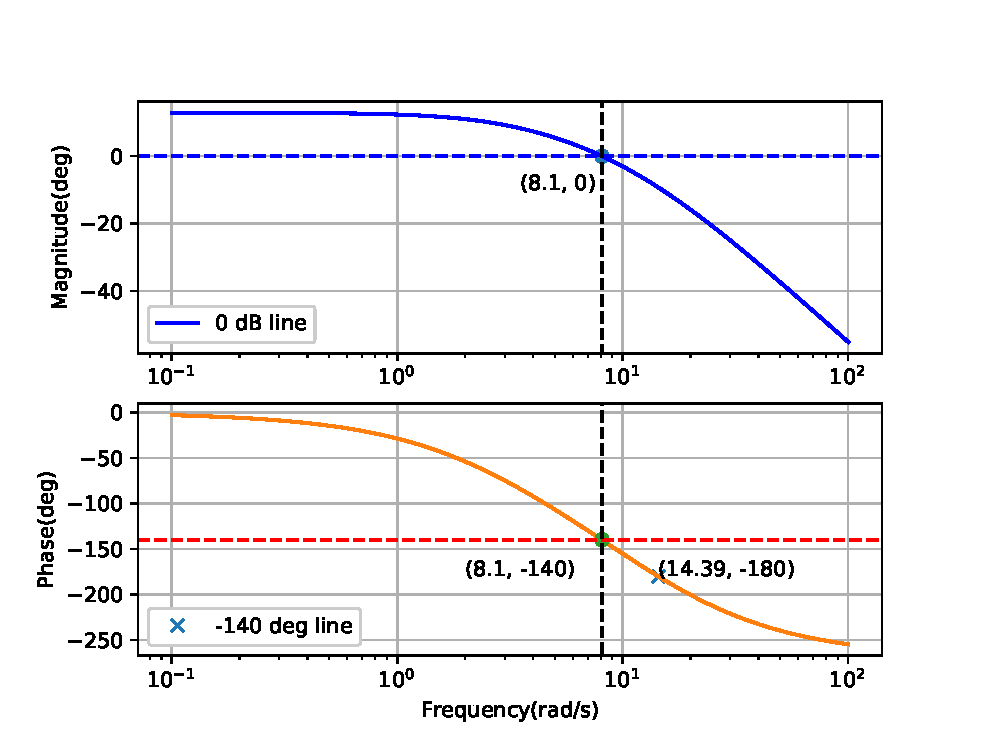
\includegraphics[width=\columnwidth]{ee18btech11033_ver2.eps}
\caption{Bode Plot of $G\brak{s}$ with $K= 1710.01$}
\label{fig:ee18btech11033_ver2}
\end{figure}

\item $\brak{iii}$ 20 percent peak overshoot in step response.
\\
\solution 
\begin{align}
    \frac{G\brak{s}}{1+G\brak{s}} \quad \quad \quad\quad\quad
    \\
    \ = \frac{K}{s^3 + 27s^2 + 207s + \brak{405+K}} &= Y\brak{s}
\end{align}
Step response-
\begin{align}
    \frac{K}{\brak{s}[s^3 + 27s^2 + 207s + \brak{405+K}]}
\end{align}
By final value theorem, steady state value-

\begin{align}
    \lim_{s \to 0} sY\brak{s} = \lim_{t \to \infty} y\brak{t} = \frac{k}{405}
\end{align}
So the value at peak should be $\frac{6k}{2025}$.
Now it is extremely difficult to find K  from the given data.
Since it a Third order system, there exist no explicit formula for peak time. Thus, trying a random value of K under the bound the satisfies routh hurwitz, then taking inverse Laplace and differentiating to get peak time and thus overshoot, is the only method that remains.
 
\end{enumerate}
